\section{Espectro de señales}

\subsection{sinc}

En esta experiencia se estudió el espectro de una señal sinc con una amplitud de $350 mVpp$ (medidos con el OUT TERM en HiZ) y una frecuencia de $100 kHz$. En la figura \ref{fig:osc} se puede observar la señal sinc en el osciloscopio, mientras que en \ref{fig:sinc} se observa el espectro visto en el analizador. El resultado coincide con lo esperado, pues la transformada de Fourier del sinc es, en efecto, un pulso.

\begin{figure}[H]
	\centering
	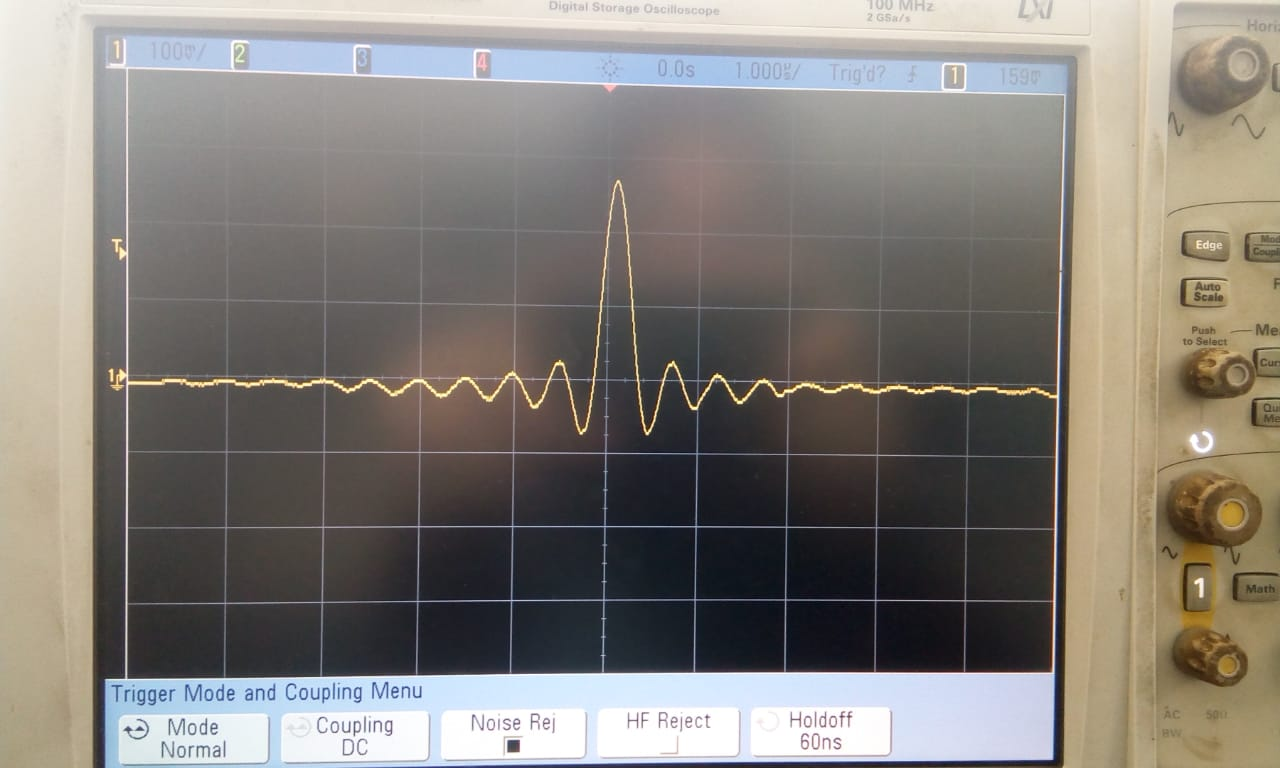
\includegraphics[width=0.9\textwidth]{/ImagenesEjercicio8/sinc8.jpeg}
	\caption{Señal sinc vista en el osciloscopio}	
	\label{fig:osc}
\end{figure}

\begin{figure}[H]
	\centering
	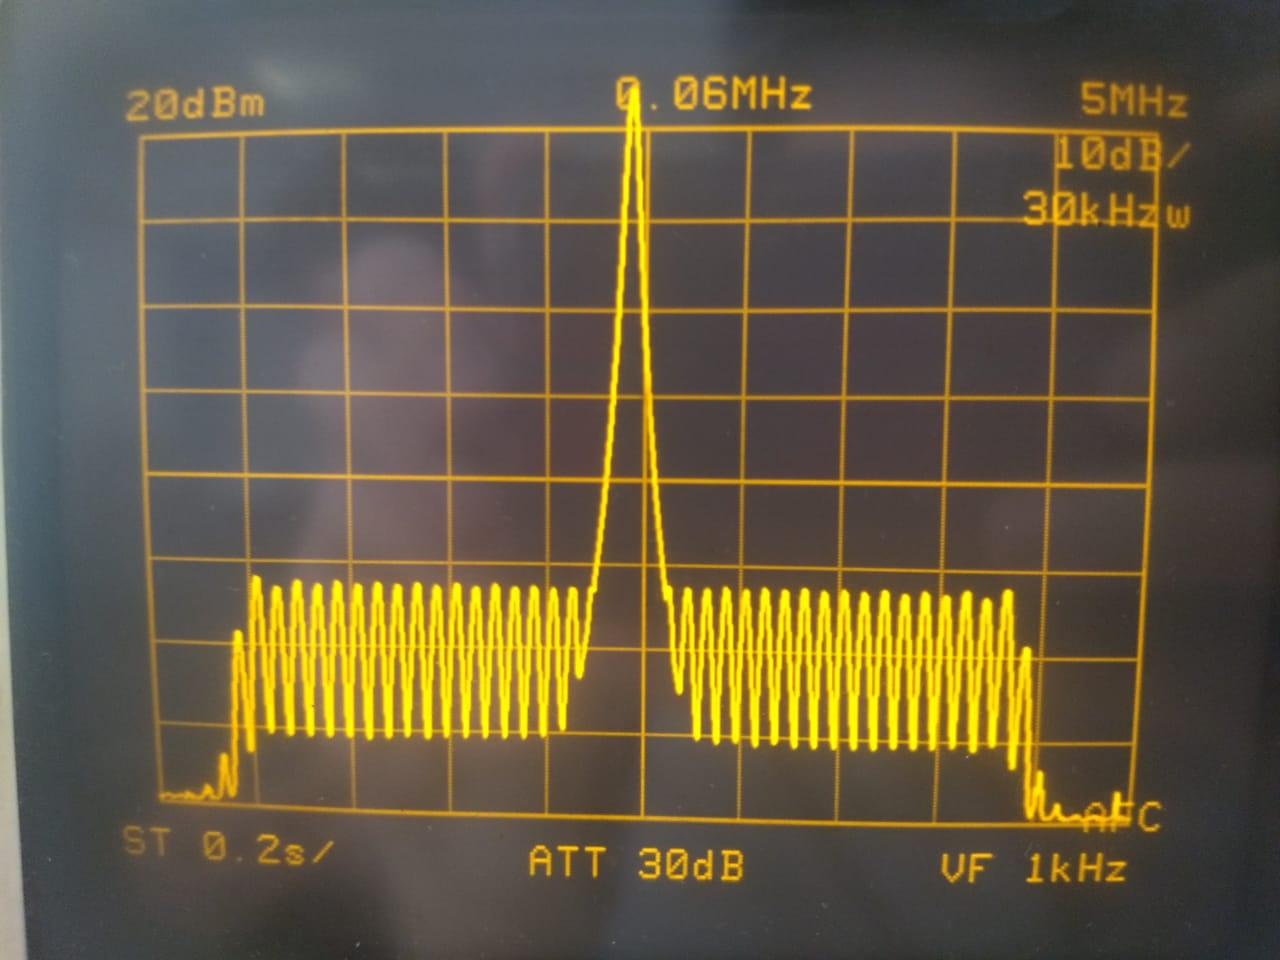
\includegraphics[width=0.9\textwidth]{/ImagenesEjercicio8/sinc2.jpeg}
	\caption{Espectro de la señal sinc}	
	\label{fig:sinc}
\end{figure}

\subsection{Tren del deltas}

En esta parte se estudió el espectro de un tren de deltas, con la misma configuración en amplitud y frecuencia que la señal del ejercicio anterior. Para configurar el tren de deltas, se formó un tren de pulsos con DC mínimo, que con el generador utilizado se tradujo en un DC del 20\% En la figura \ref{fig:del} se puede apreciar el espectro observado.

\begin{figure}[H]
	\centering
	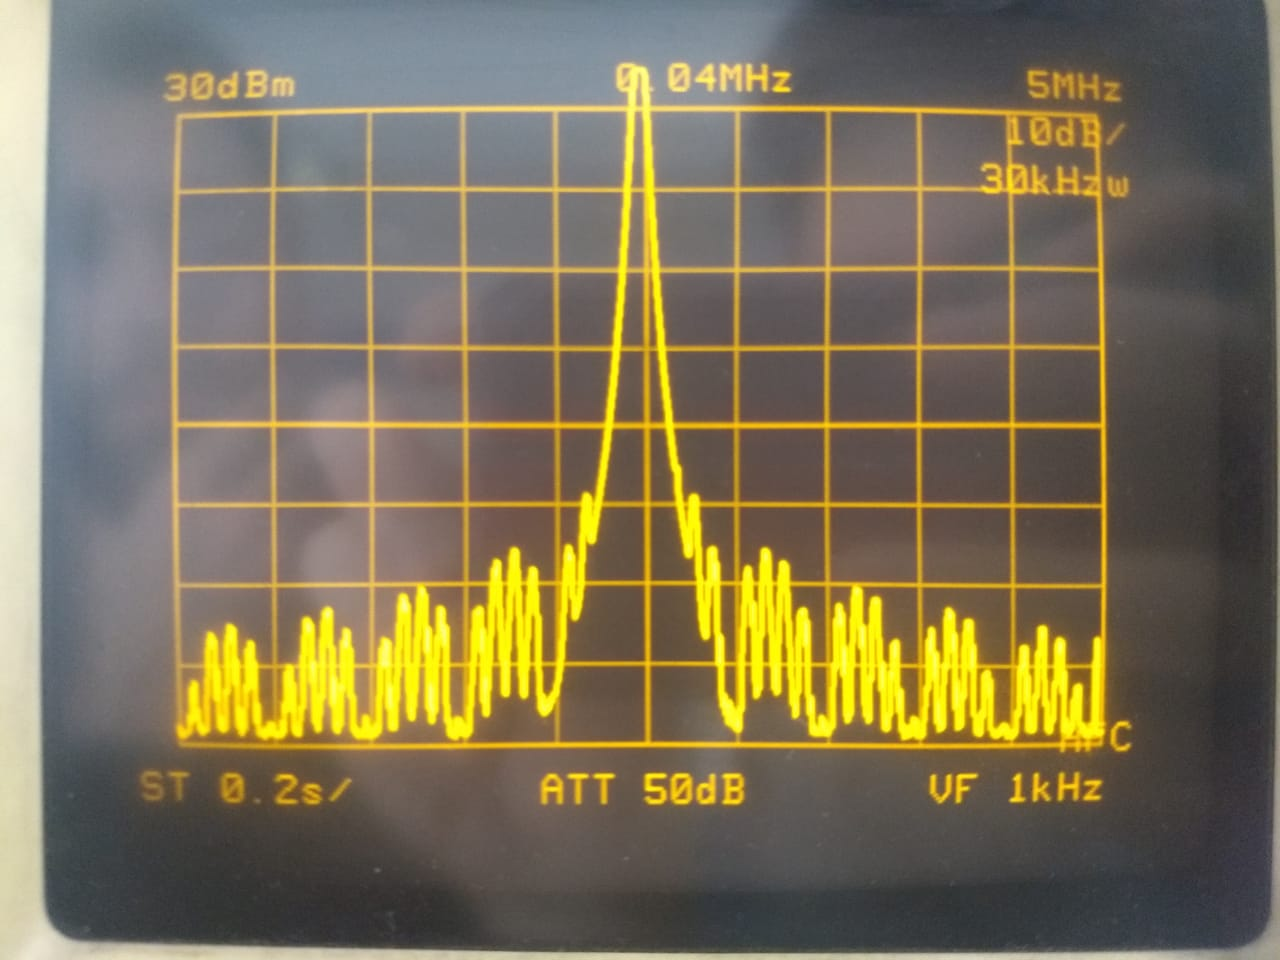
\includegraphics[width=0.9\textwidth]{/ImagenesEjercicio8/trendeltas1.jpeg}
	\caption{Espectro del tren de deltas}	
	\label{fig:del}
\end{figure}

El espectro se asemeja más a un sinc que al tren de deltas que se esperaría observar. La posible causa de esto es que al no ser lo suficientemente pequeño el duty cycle no se logre generar algo parecido a un tren de deltas a la entrada, de donde lo que se observa es más similar al espectro de un tren de pulsos que a uno de deltas.
